%************************************************
\chapter[Appendix 5.1: Chapter 5 - Supplementary results]{Appendix 5.1: Chapter 5 - Supplementary results}\label{ch:spatial_appendix}
%************************************************

\renewcommand{\thefigure}{A.5.1.\arabic{figure}}
\setcounter{figure}{0}

\renewcommand{\thetable}{A.5.1.\arabic{table}}
\setcounter{table}{0}

Here we show the response of the studied metrics in relationship to variability in the dispersal and foraging rates (\(d\) and \(f\), which are both fixed to \(0.5\) in the main simulations). We performed supplementary simulations in which we varied both rates in the interval \([0.25,0.75]\). In the simulations accounting for both dispersal and foraging, we also simulated communities with high values of dispersal rates and low foraging rates, and viceversa.

The ratio of positive to negative interactions (left panel of Fig. \ref{fig:figApp5.1}) varies from 0.94 to 1.05, with the highest variability being observed in the inter-patch effects of the dispersal simulation and the intra-patch effects of the foraging one. The magnitude of the net effects is much more variable for intra-patch effects than for inter-patch ones (middle panel of Fig. \ref{fig:figApp5.1}), with its average value being in all cases relatively close to zero, which invites the interpretation that, regardless of the parameterization chosen, positive and negative net effects tend to mirror each other in number and also in magnitude. The number of pairwise interactions that switch sign from direct to net effect (right panel of Fig. \ref{fig:figApp5.1}) is lowest in the dispersal simulations, but these also show the highest variability, in the local, intra-patch, interactions. Simulations with foraging and with both movement types are less variable and, in all cases, the frequency of sign switches between populations of different locations is lower than the frequency of switches between populations of the same location.

The variations in \(d\) and \(f\) are reflected in the relationship between the magnitude of intra and inter-patch net effects (\cref{fig:fig5.2}). In the dispersal simulations, an increase in \(d\) trigger an increase in inter-patch net effects relative to intra-patch ones (Fig. \ref{fig:figApp5.2}, three upper panels). In the foraging configuration, higher inter-patch foraging triggers a higher variability in both intra-patch and inter-patch effects, with no apparent directionality, whereas low \(f\) values clearly reduce the magnitude of inter-patch effects, as expected. The simulations with both dispersal and foraging show a mixture of the patterns described above; it is worth noting that even a small addition of foraging is able to scatter the packed configuration of dispersal-only net effects of the upper panels of Fig. \ref{fig:figApp5.2}.

The spatial decay of net effects is quite similar across parameterizations (Fig. \ref{fig:figApp5.3} and Fig. \ref{fig:figApp5.4}). Interestingly, for high values of inter-patch dispersal or foraging, the spatial cascades do not generally increase in length or in the magnitude of the effect at a given length (compare middle and right panels of Fig. \ref{fig:figApp5.3} and Fig. \ref{fig:figApp5.4}). On the other hand, low values of \(d\) or \(f\) do induce lower net effects across the spatial cascades generated (compare middle and left panels of Fig. \ref{fig:figApp5.3} and Fig. \ref{fig:figApp5.4}, note the variation in vertical axis). This asymmetrical effect could be due to the design and parameterization of the model or reflect an underlying ecological process of effect dampening at high direct interaction strengths.

\begin{figure}
\centering
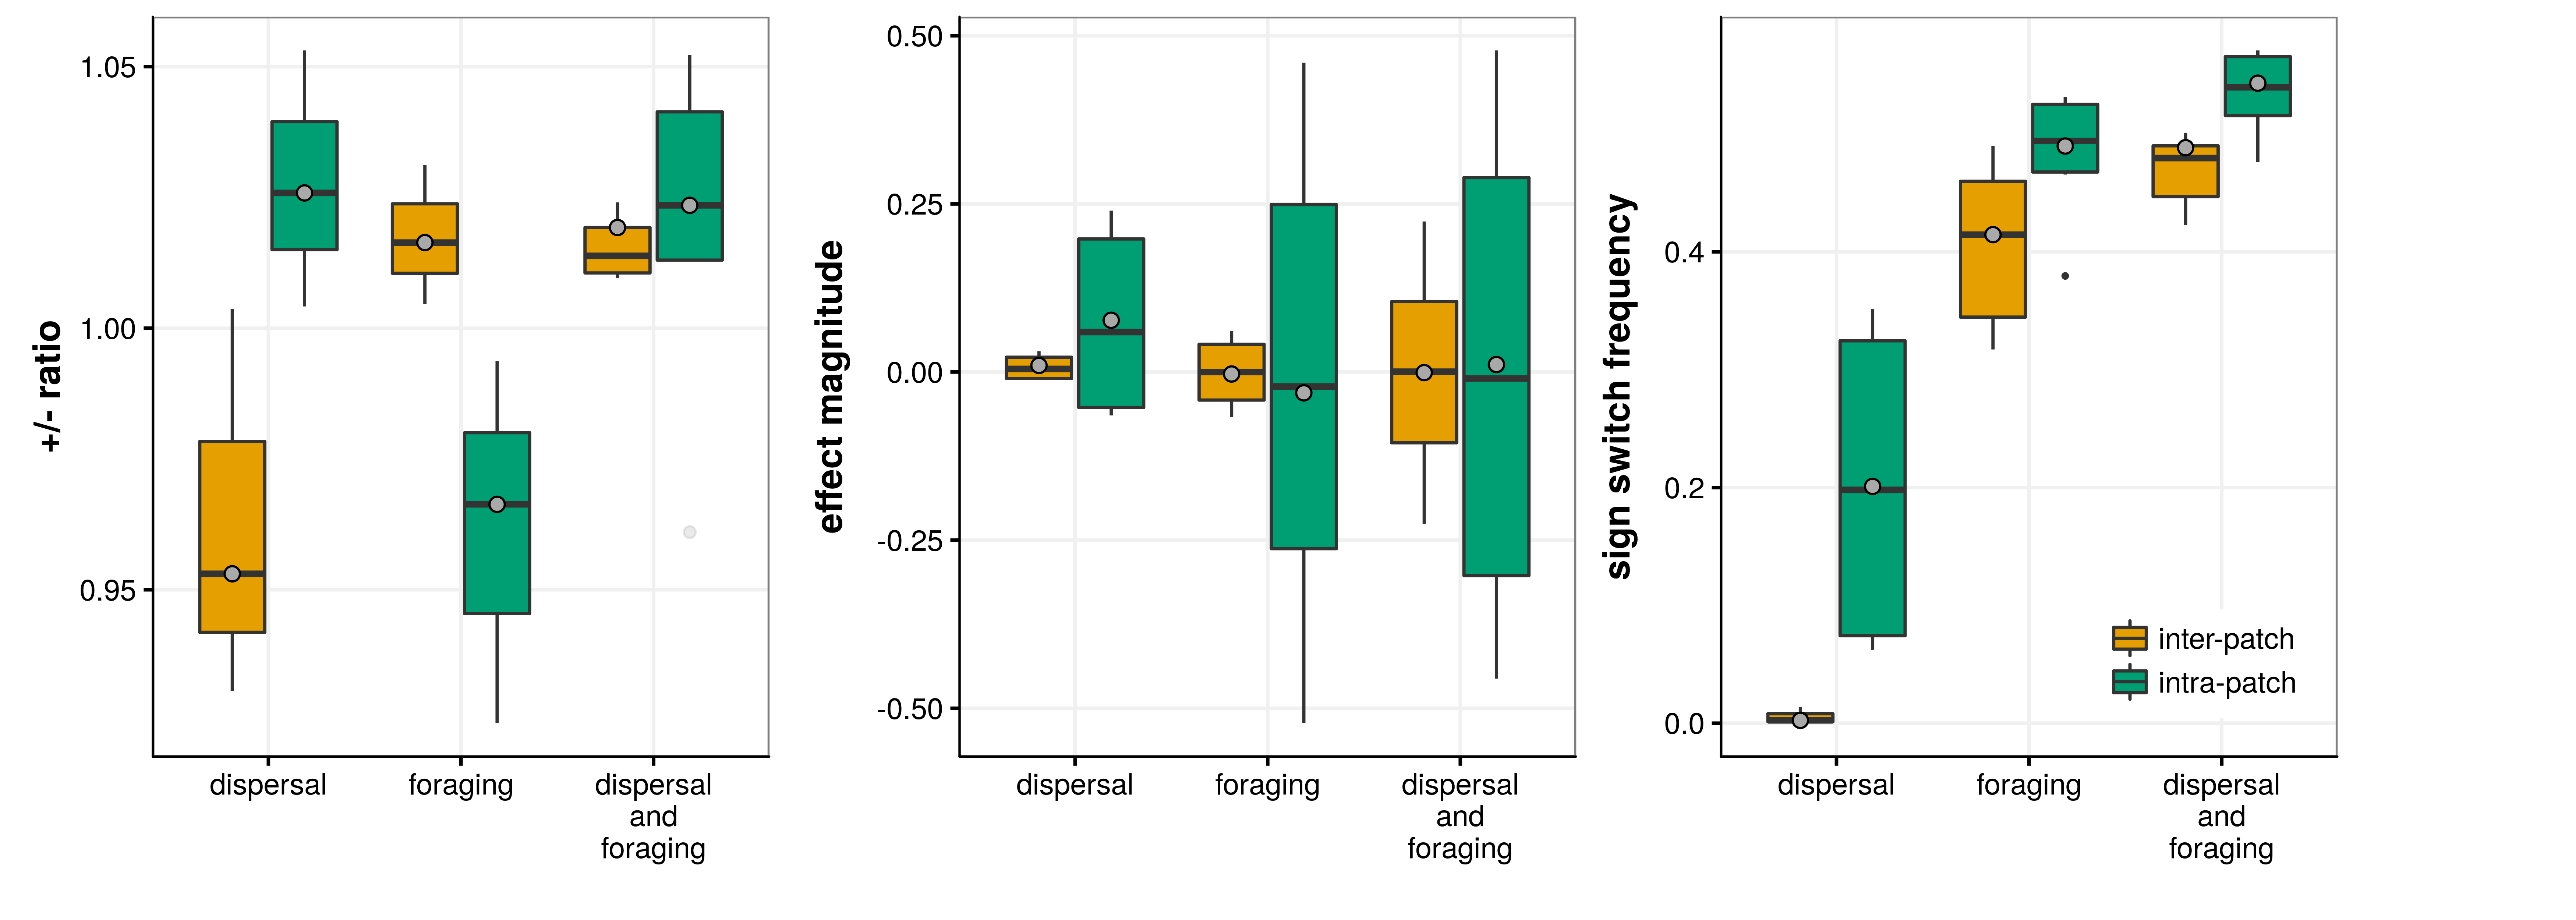
\includegraphics[width=\textwidth,height=\textheight,keepaspectratio]{./Figures/Appendix5_1/Fig_1.png}
\caption[Varying +/- ratios with $d$ and $f$]{\color{Gray}Variability in a) ratio of positive to negative net effects, b) mean net effect magnitude, and c) relative frequency of sign switches between direct and net effects, for varying dispersal and foraging rates. Grey points represent the metrics for the values of the main simulations (d = 0.5, f = 0.5) . \label{fig:figApp5.1}} \end{figure}

\newpage

\begin{figure}
\centering
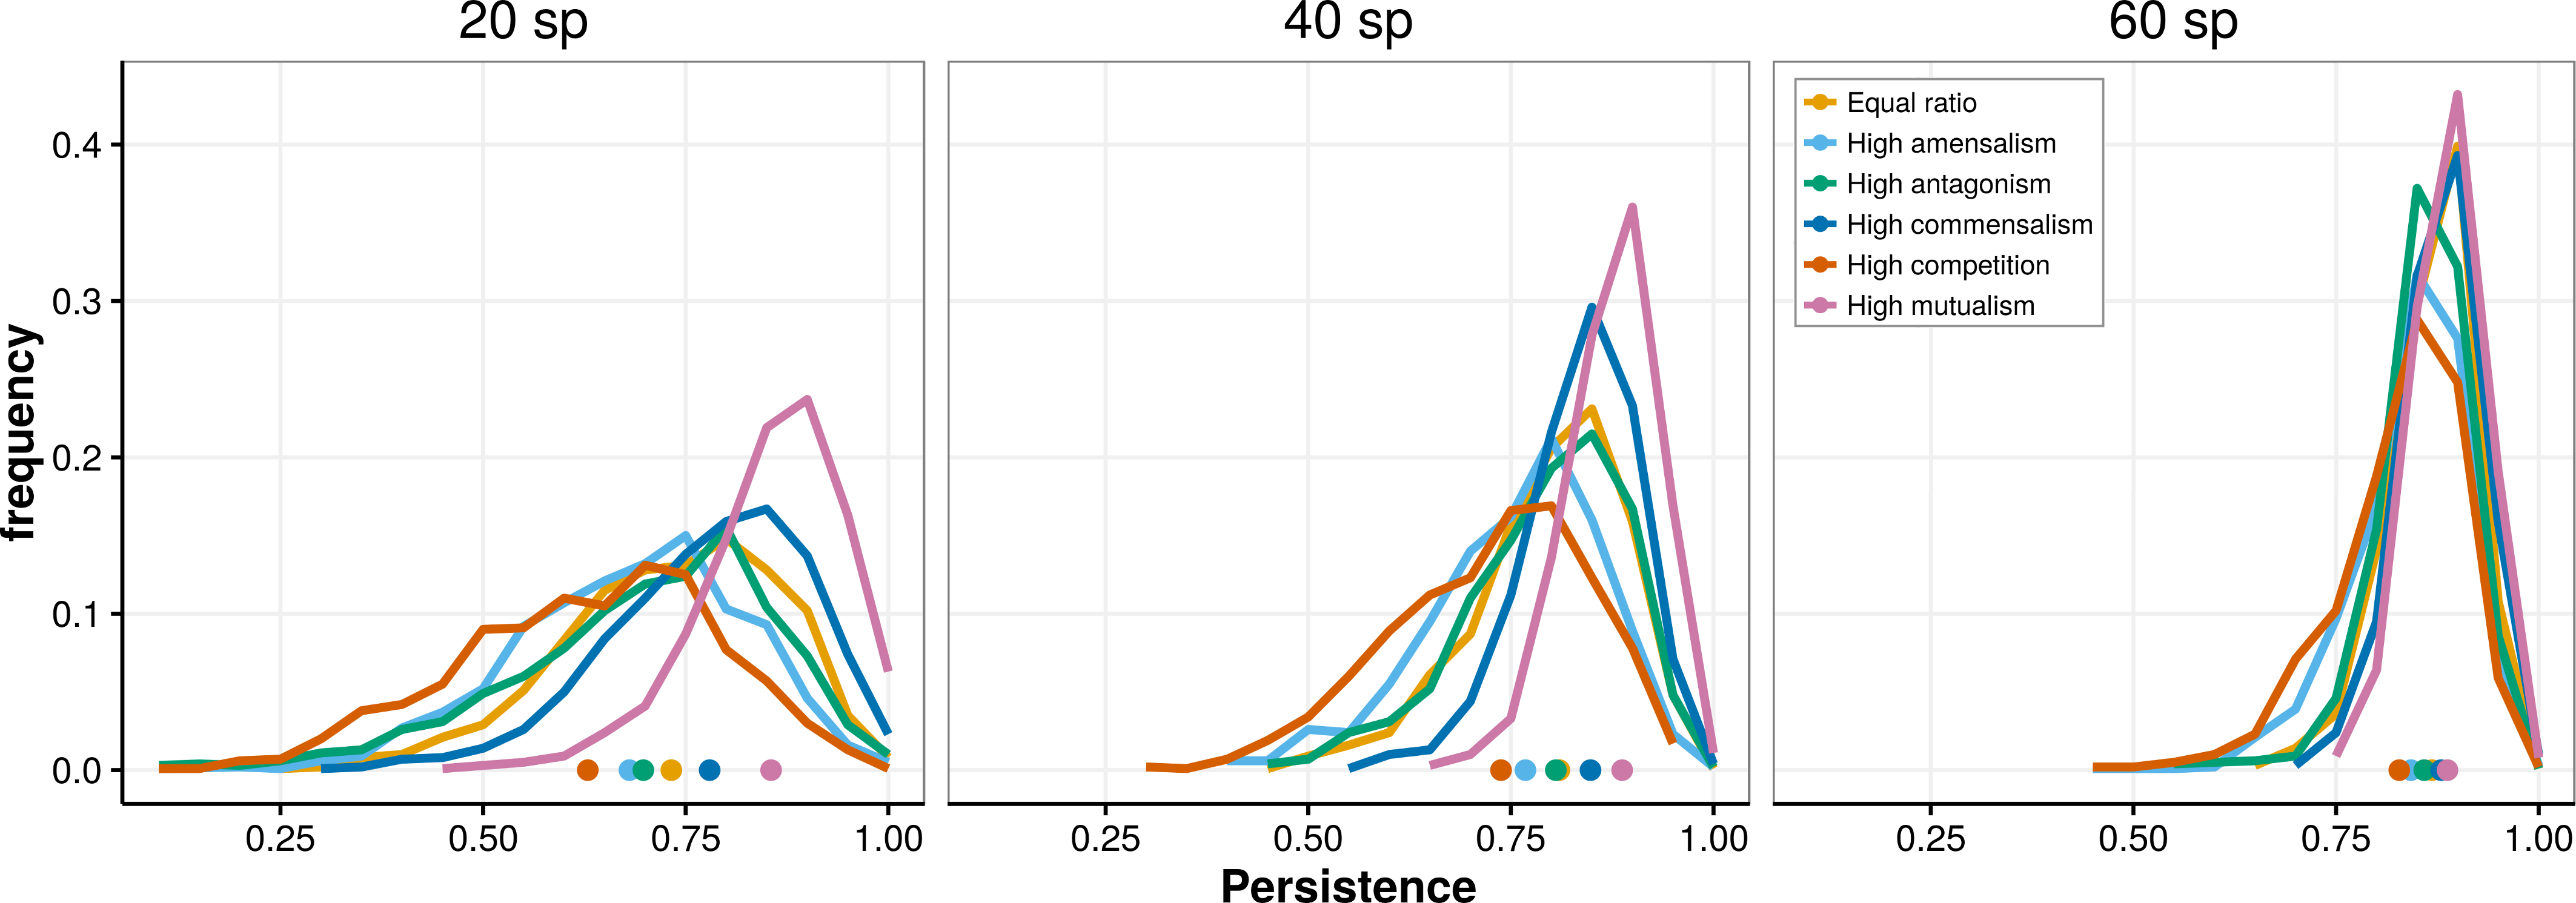
\includegraphics[width=.7\textwidth,height=\textheight,keepaspectratio]{./Figures/Appendix5_1/Fig_2.png}
\caption[Varying net effects with $d$ and $f$]{\color{Gray}Variability in across and within-patch pairwise net effects for different dispersal and foraging rates (cf \cref{fig:fig5.2} of chapter 5). In the panels, ``d'' is the dispersal rate, ``f'' foraging rate, ``low'' indicates a value of 0.25, ``intermediate'' 0.5, and ``high'' 0.75. Note that ``intermediate'' values correspond to the parameterization of the main simulations. \label{fig:figApp5.2}}
\end{figure}

\newpage

\begin{figure}
\centering
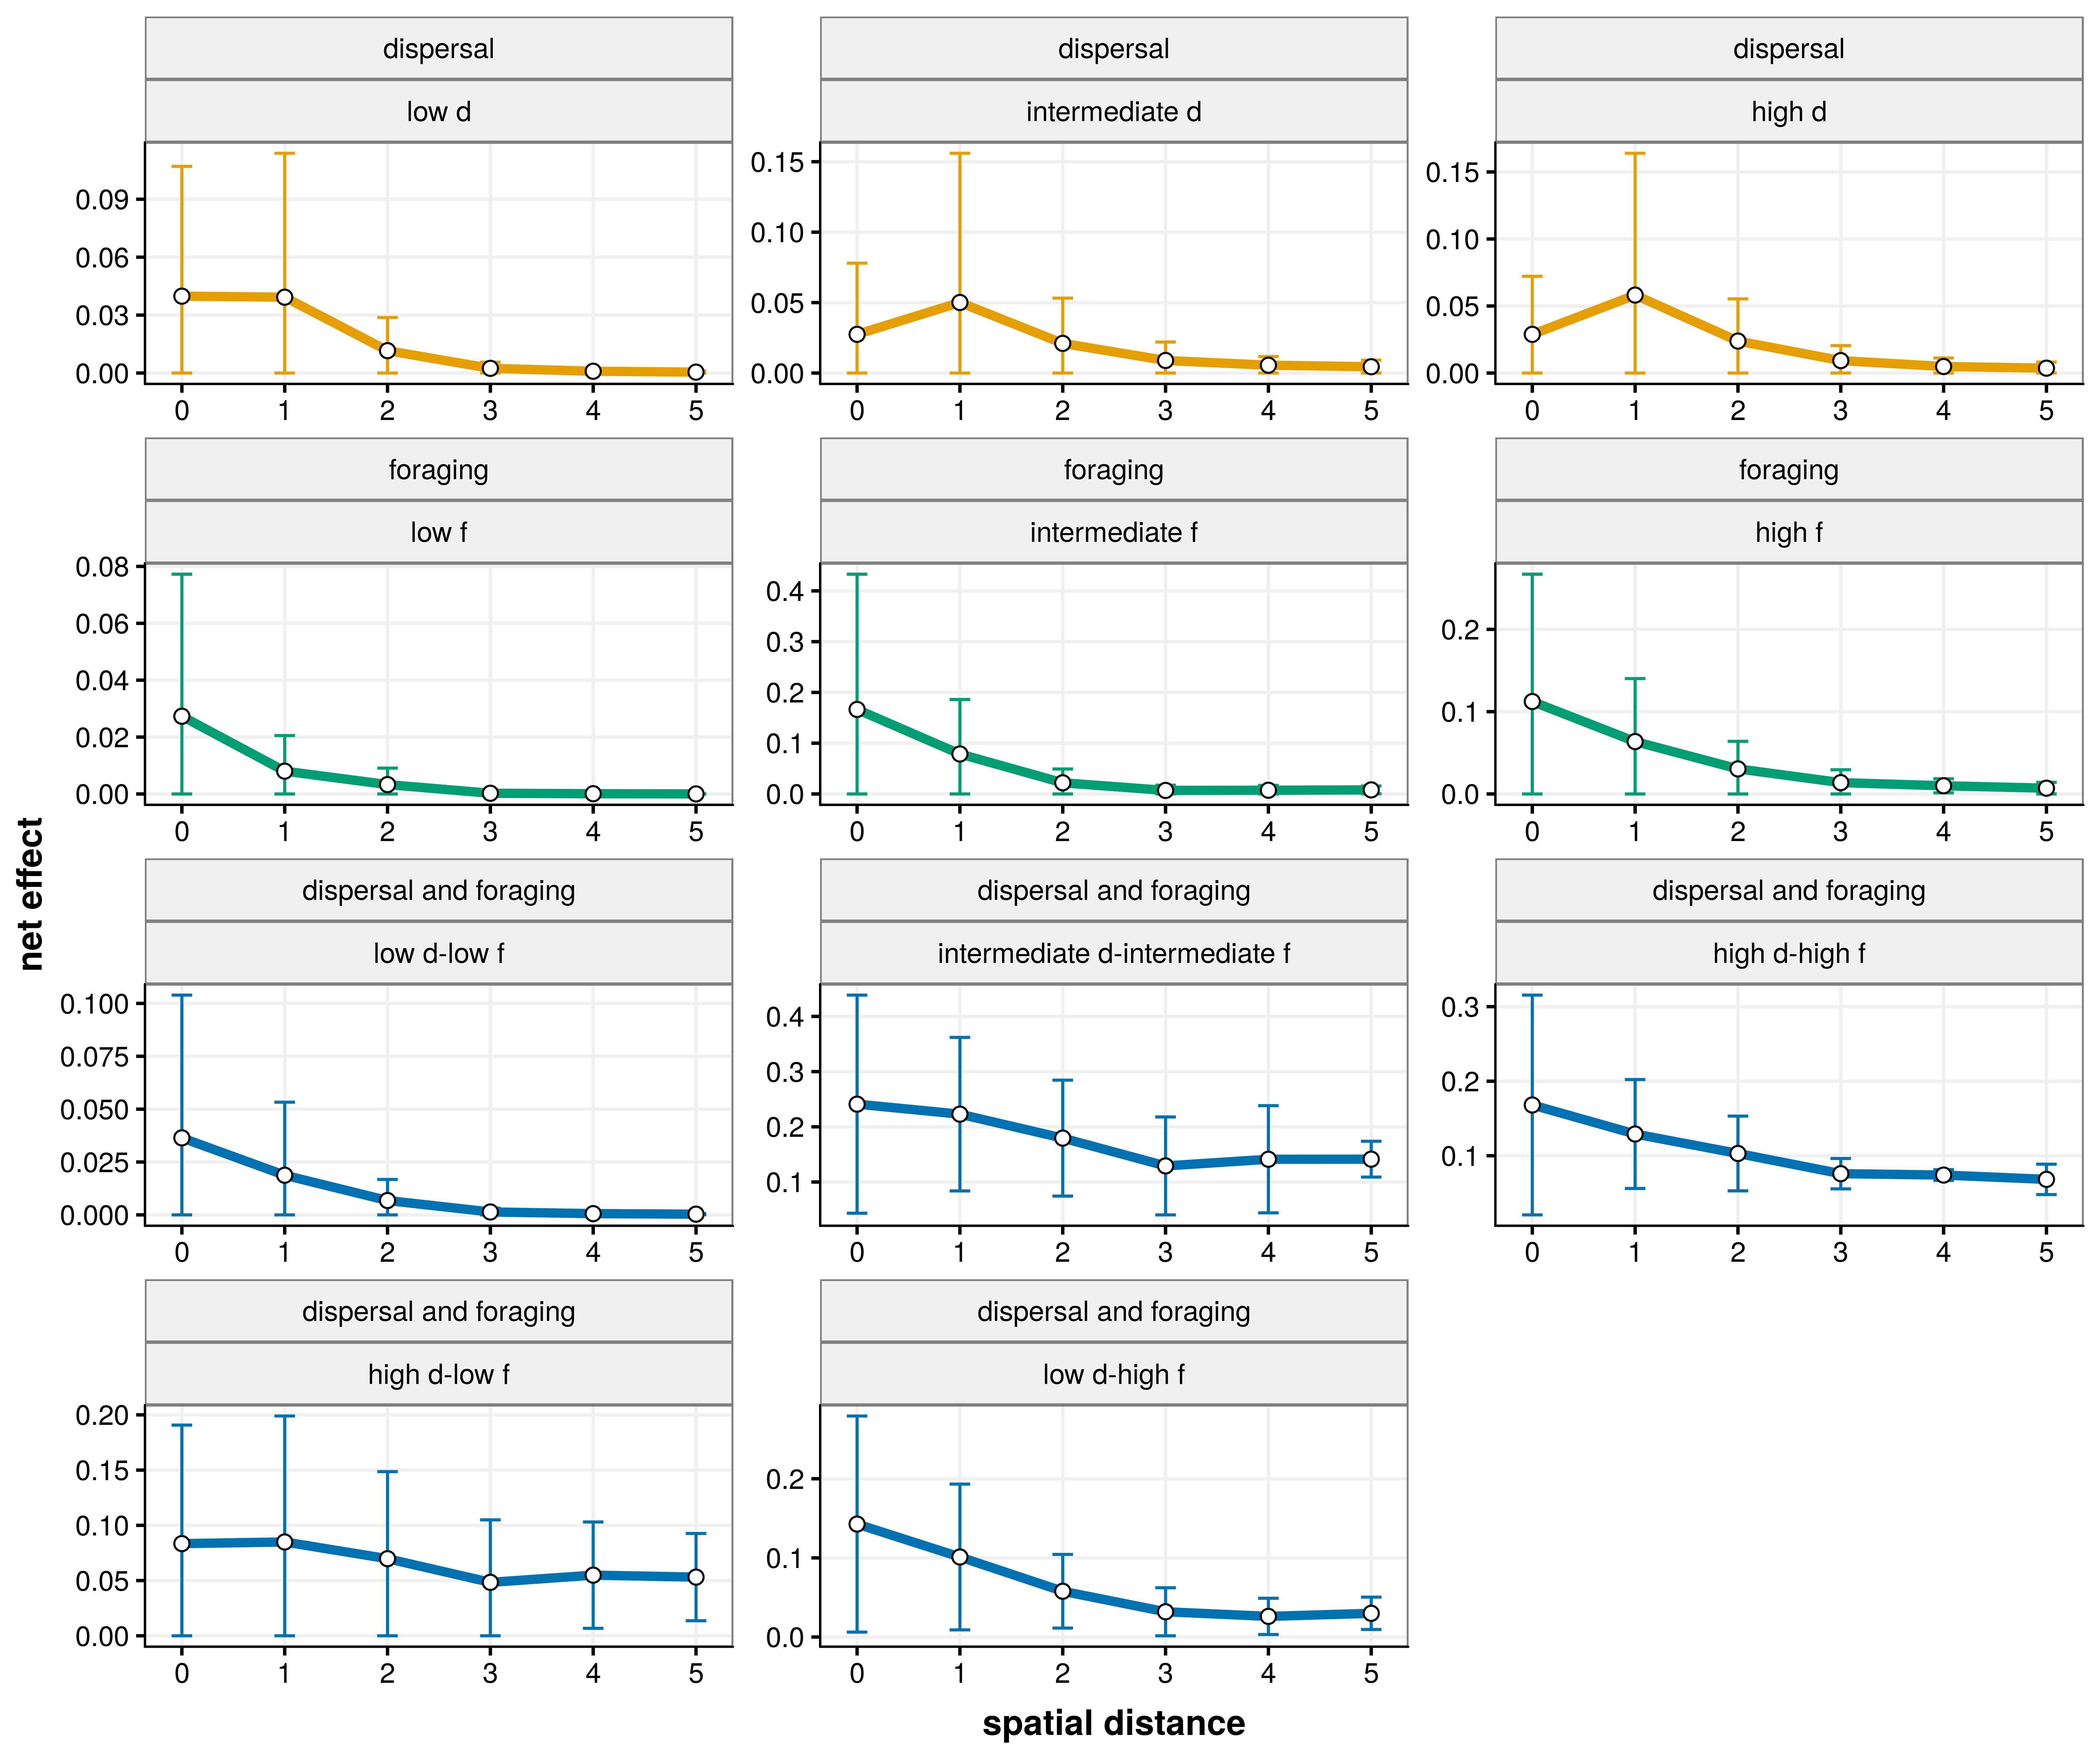
\includegraphics[width=\textwidth,height=\textheight,keepaspectratio]{./Figures/Appendix5_1/Fig_3.png}
\caption[Varying spatial decay with $d$ and $f$]{\color{Gray} Variability in the relationship between net effect and spatial distance for different dispersal and foraging rates (cf panel a of \cref{fig:fig5.3} in chapter 5). Panel legend as in Fig. \ref{fig:figApp5.2} \label{fig:figApp5.3}}
\end{figure}

\newpage

\begin{figure}
\centering
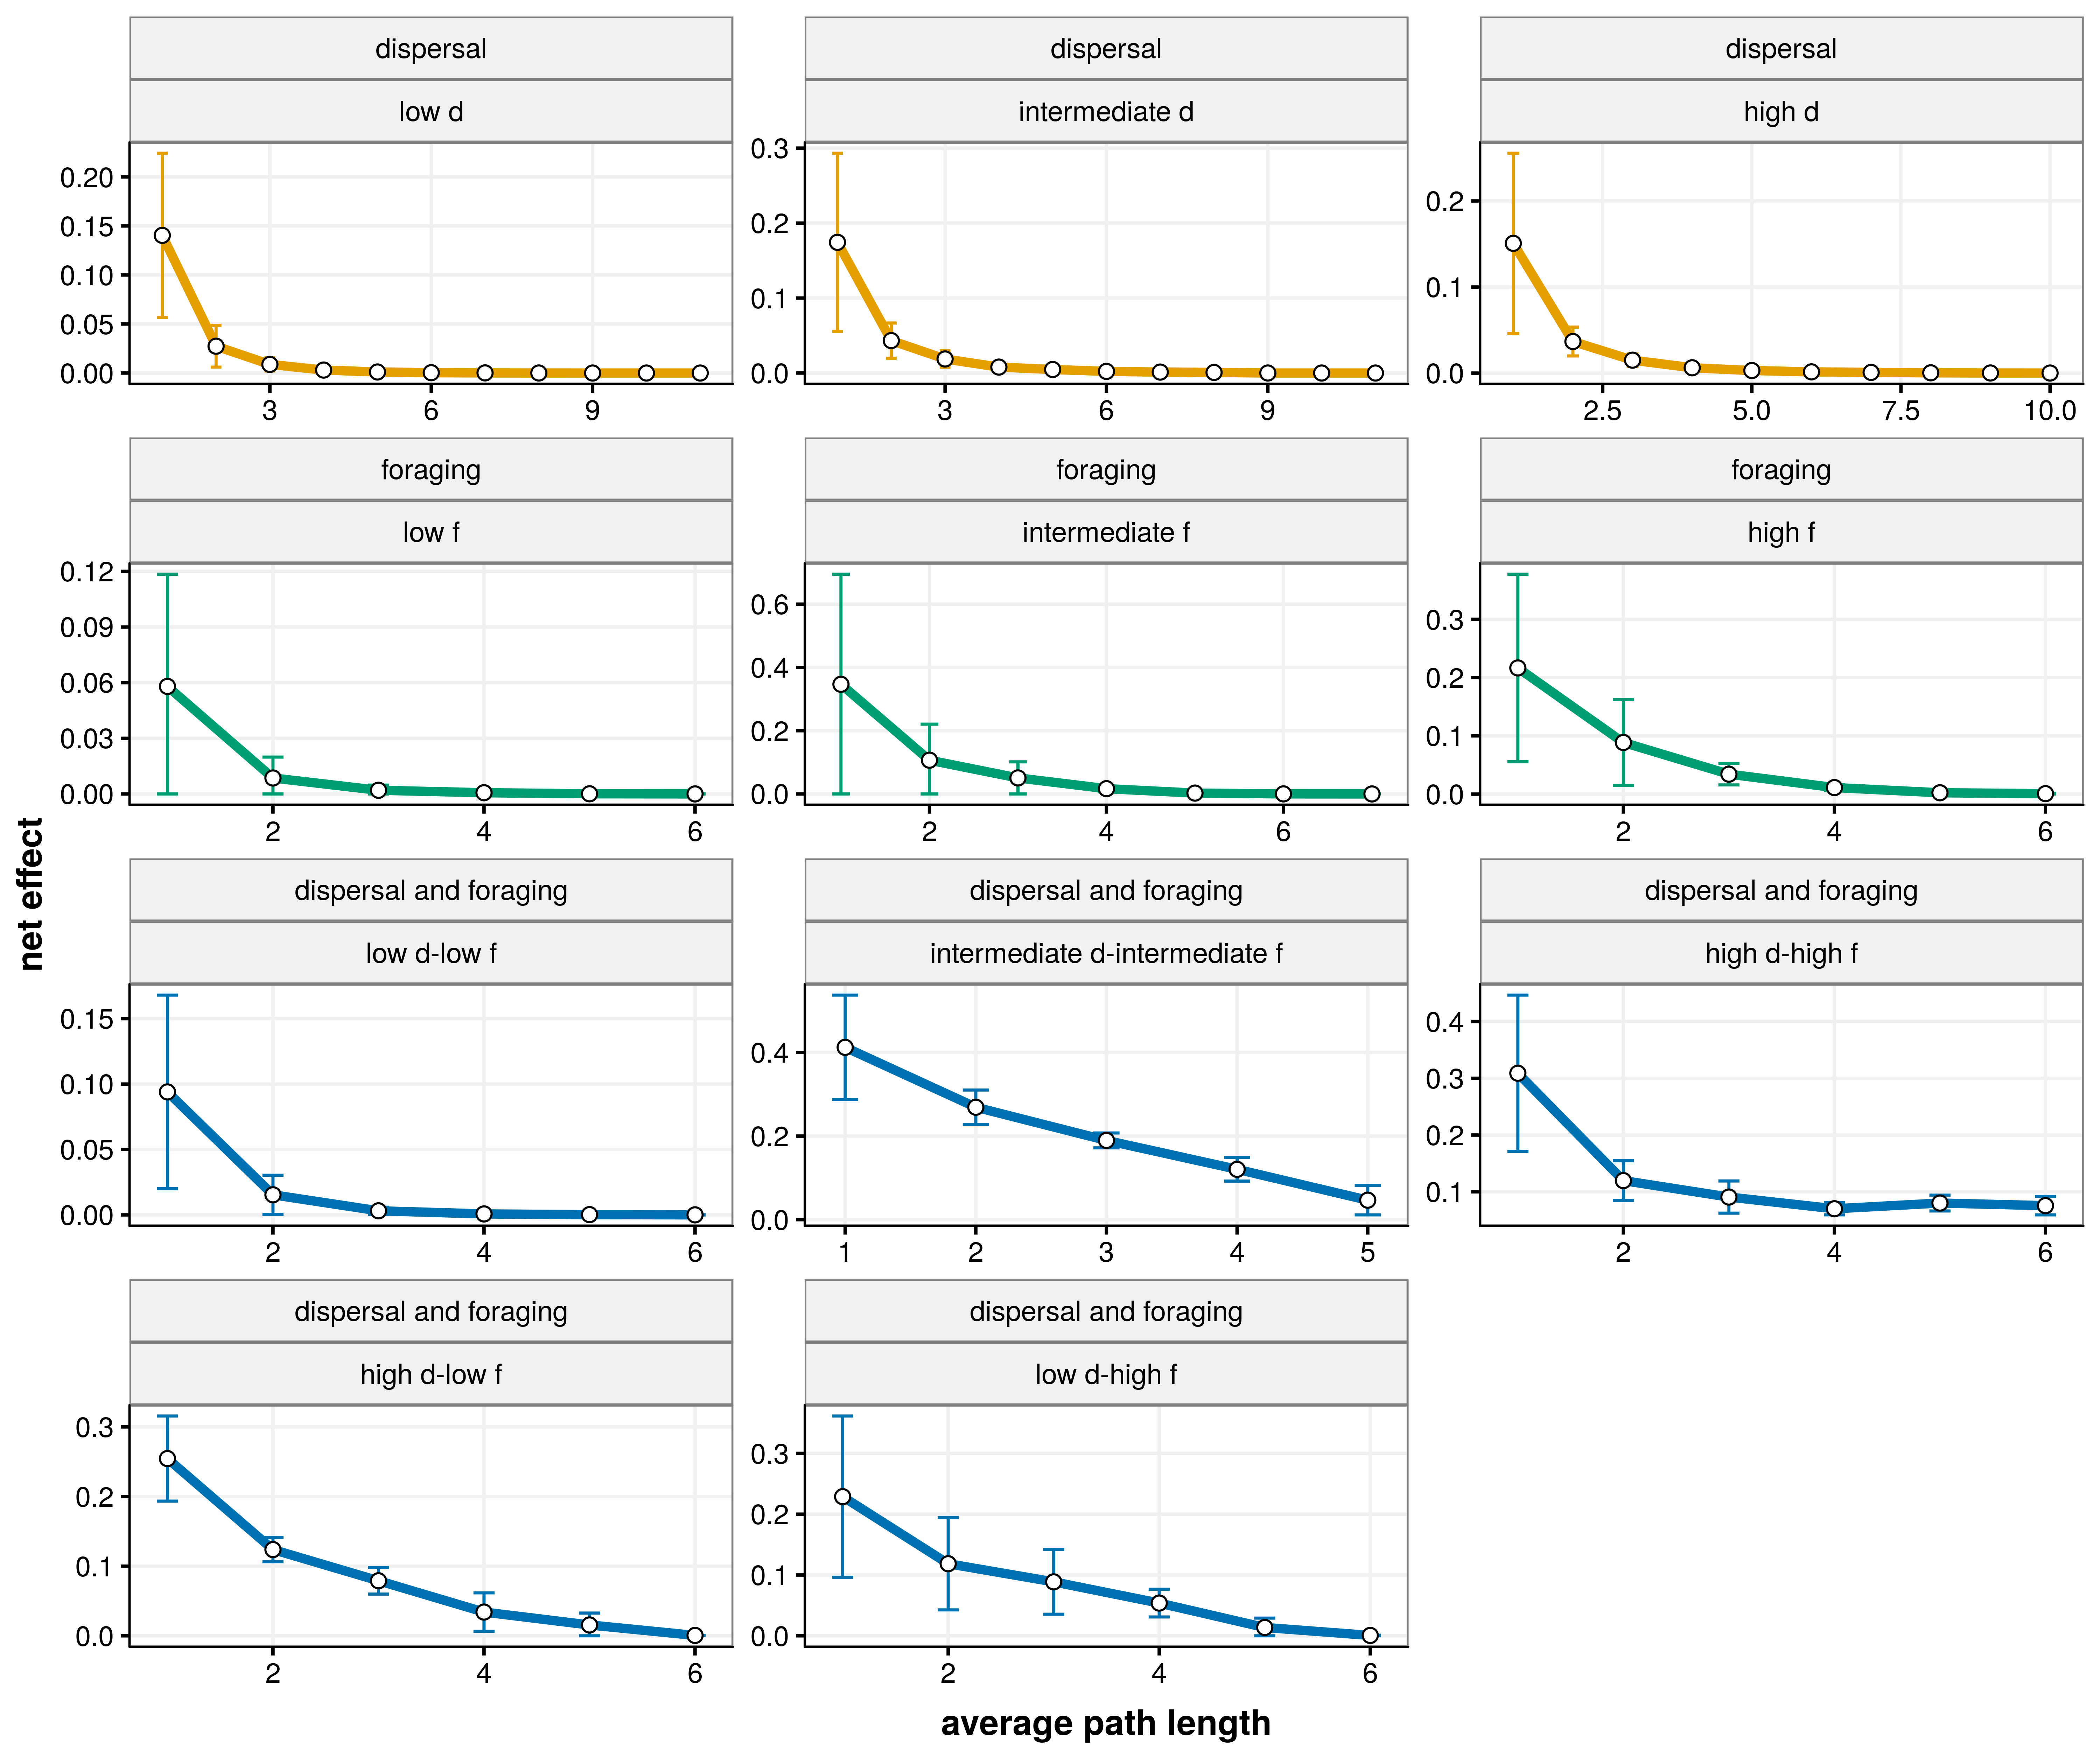
\includegraphics[width=\textwidth,height=\textheight,keepaspectratio]{./Figures/Appendix5_1/Fig_4.png}
\caption[Varying path length decay with $d$ and $f$]{\color{Gray} Variability in the relationship between net effect and average path length for different dispersal and foraging rates (cf. panel (b) of \cref{fig:fig5.3} in chapter 5). Panel legend as in Fig. \ref{fig:figApp5.2} \label{fig:figApp5.4}}
\end{figure}
